\chapter{Shapes}

\section{Hats}

A useful family of shapes, which can be packed into each other quite well, are rounded, non-acute triangles. We call these shapes \emph{hats}:

\begin{definition}
    For each $0 \le b \le a$, an \emph{$(a,b)$-hat} is a non-acute triangle with an incircle of area $a$, whose corners are rounded to the radius of a $b$-circle, see \Cref{fig:hat}. Call the triangle's longest side the hat's \emph{base}, and the triangle's angles to the left and to the right of the base the triangle's \emph{right-angle} and \emph{left-angle}.
    %An $a$-hat is an $(a,0)$-hat.
    If we say \emph{right hat} or \emph{obtuse hat}, the hat is based on a right/obtuse triangle.
\end{definition}

\begin{figure}[htbp!]
    \centering

    \begin{tikzpicture}[scale=3]
        \hatsimple{\defaulta}{\defaultb}{\defaultr}
    \end{tikzpicture}

    \caption{An $(a,b)$-hat.}
    \label{fig:hat}
\end{figure}

\begin{definition}\label{def:hat-split-key}
    A hat's \emph{associated split key} equals the tuple of the areas of the two circles incribed in the hat's two sides when splitting the underlying triangle orthogonally to its base through its tip, see \Cref{fig:hatf}.
\end{definition}

\begin{figure}[htbp!]
    \centering

    \begin{tikzpicture}[scale=3]
        \hatf{\defaulta}{\defaultb}{\defaultr}
    \end{tikzpicture}

    \caption{A hat's \emph{associated split key} equals $(f_1, f_2)$}
    \label{fig:hatf}
\end{figure}

%%For the following proofs, we need to know a hat's dimensions in detail. We construct these measures using \Cref{fig:construction}.
%%
%%\begin{lemma}\label{lm:sizes}
%%    Let $r$ be the radius of an $a$-circle, and $s$ be the radius of a $b$-circle.
%%
%%    A ($a,b$)-hat has
%%    \begin{itemize}
%%        \item height $h(a) = \textcolor{blue}{r + r\s} = \sqrt{\frac a \pi}(1+\s)$,
%%        \item width $w(a,b) = 2\textcolor{blue}{(r+r\s)} - 2\textcolor{orange}{s\s} = \sqrt{\frac a \pi}(2+2\s)-\sqrt{\frac b \pi}2\s$,
%%        \item and diagonal $d(a,b) = \textcolor{red}{(r+r\s)\s} - \textcolor{orange}{s\s} = \sqrt{\frac a \pi}(2+\s)-\sqrt{\frac b \pi}\s$.
%%    \end{itemize}
%%
%%    We define two additional measures for the case when one of the corners is not rounded:
%%    \begin{itemize}
%%        \item corner-width $w'(a,b) = w(a,b) + \textcolor{orange}{s\s} = \sqrt{\frac a \pi}(2+2\s)-\sqrt{\frac b \pi}\s$,
%%        \item and corner-diagonal $d'(a) = d(a,0) = \sqrt{\frac a \pi}(2+\s)$.
%%    \end{itemize}
%%\end{lemma}
%%
%%\begin{figure}[htbp!]
%%    \centering
%%
%%    \begin{tikzpicture}[scale=4]
%%        \hatconstruction
%%    \end{tikzpicture}
%%
%%    \caption{Constructing the dimensions of an $(a,b)$-hat.}
%%    \label{fig:construction}
%%\end{figure}
%%

\begin{lemma}\label{th:hatsinhat}
    Consider an $(a,0)$-hat with the associated split key $F = (f_1, f_2)$, and call its left- and right-angles $\alpha$ and $\beta$.
    For all $(F,0)$-rounded tuples $(a_1, b_1)$ and $(a_2, b_2)$ with $a_1 + a_2 \le a$, the following two shapes can be packed into the hat:
    \begin{itemize}
        \item A right $(a_1,b_1)$-hat with a right-angle of $\alpha$ and
        \item a right $(a_2,b_2)$-hat with a left-angle of $\beta$.
    \end{itemize}
\end{lemma}

\begin{proof}
    Place the hats' tips at the bottom of the container hat, rotate their $\alpha$- and $\beta$-angles towards the container's matching angles and push them as far to the left/right as possible. Figure \Cref{fig:hatsinhat} shows examples how this packing looks like for different values of $a_1$ and $a_2$.

    \begin{figure}[htbp!]
        \centering

        \begin{tikzpicture}[scale=2]
            \hatsinhat{\defaulta}{\defaultb}{0}{0}
        \end{tikzpicture}
        \begin{tikzpicture}[scale=2]
            \hatsinhat{\defaulta}{\defaultb}{0.5}{0}
        \end{tikzpicture}

        \vspace{2mm}

        \begin{tikzpicture}[scale=2]
            \hatsinhat{\defaulta}{\defaultb}{0.1}{0}
        \end{tikzpicture}
        \begin{tikzpicture}[scale=2]
            \hatsinhat{\defaulta}{\defaultb}{0.7}{0}
        \end{tikzpicture}

        \vspace{2mm}

        \begin{tikzpicture}[scale=2]
            \hatsinhat{\defaulta}{\defaultb}{0.2}{0}
        \end{tikzpicture}
        \begin{tikzpicture}[scale=2]
            \hatsinhat{\defaulta}{\defaultb}{0.9}{0}
        \end{tikzpicture}

        \vspace{2mm}

        \begin{tikzpicture}[scale=2]
            \hatsinhat{\defaulta}{\defaultb}{0.4}{0}
        \end{tikzpicture}
        \begin{tikzpicture}[scale=2]
            \hatsinhat{\defaulta}{\defaultb}{1}{0}
        \end{tikzpicture}

        \caption{Hat-in-hat packings for different values of $a_1$ and $a_2$}
        \label{fig:hatsinhat}
    \end{figure}

    This placement constitutes a valid packing if (1) the hats do not overlap each other and (2) the hats fit into the hat individually. We are going to proof these two properties separately.

    \begin{itemize}
        \item[(1)]
            We want to show that the hats do not overlap each other.

            We first normalize the container hat's width to 1 and make an observation about the partial widths $l$ and $r$ in \Cref{fig:hatlr}: If the top angle is a right angle, the partial widths have the same lengths as the triangle's two cathetus $x$ and $y$ (TODO is it clear why?), so by Pythagoras, $l^2 + r^2 = 1$. If the top angle is more obtuse, but the incircle's center stays at the same $x$-coordinate (like the dotted variant), both $l$ and $r$ shrink, so for each hat, $l^2 + r^2 \le 1$, or $r \le \sqrt{1-l^2}$.

            \begin{figure}[htbp!]
                \centering

                \begin{tikzpicture}[scale=3]
                    \hatlr{\defaulta}{\defaultb}{39}{51}
                \end{tikzpicture}

                \caption{$l^2 + r^2 \le 1$ holds for each non-acute triangle}
                \label{fig:hatlr}
            \end{figure}

            The two hats do not overlap if their incircles do not overlap. If we enclose their incircles with hats which are \emph{similar} to the container, like in \Cref{fig:hatsoverlap}, we see that they do not overlap if the following condition holds:

            \begin{equation}\label{eq:trifit}
                lf + rg \le w
            \end{equation}

            \begin{figure}[htbp!]
                \centering

                \begin{tikzpicture}[scale=3]
                    \hatsoverlap{\defaulta}{\defaultb}{\defaultx}{0}
                \end{tikzpicture}

                \caption{$f^2 + g^2 \le w^2$ for each non-acute triangle}
                \label{fig:hatsoverlap}
            \end{figure}

            Also note that for similar hats, the ratio between their incircle's area and the square of their widths is constant (TODO clear why?). This means that if $a_1 + a_2 \le a$, then $f^2 + g^2 \le w^2$. Thus, $g \le \sqrt{w^2-f^2}$.

            Putting it all together, we can show that \Cref{eq:trifit} is true:

            \begin{align*}
                lf + rg
                &\le lf + \sqrt{1-l^2} \sqrt{w^2-f^2}\\
                &= lf + \sqrt{(1-l^2)(w^2-f^2)}\\
                &= lf + \sqrt{w - \textcolor{blue}{l^2w^2} - \textcolor{blue}{f^2} + l^2f^2}\\
                &\le lf + \sqrt{w - \textcolor{orange}{2lwf} + l^2f^2}\addtocounter{equation}{1}\tag{\theequation}\label{eq:am-gm}\\
                &= lf + \sqrt{(w-lf)^2}\\
                &= w
            \end{align*}

            Line \ref{eq:am-gm} is a consequence of the inequality of arithmetic and geometric means: $\frac{lw+f}{2} \ge \sqrt{lwf} \Rightarrow \frac{(lw+f)^2}{4} \ge lwf \Rightarrow l^2w^2 + 2 lwf + f^2 \ge 4 lwf \Rightarrow \textcolor{blue}{l^2w^2 + f^2} \ge \textcolor{orange}{2lwf}$.

        \item[(2)]
            It is left to show that the hats fit inside the container individually.

            If a hat's incircle is not larger than the incircle of the container hat's side, it will fit inside without question (like all the non-rounded hats in \Cref{fig:hatsinhat}).

            So let us assume $a_i > f_i$. For this proof, normalize the container hat's incircle to 1. Again, for hats similar to the container hat's right side, the ratio between the square root of its incircle's area and the length of its base is constant. We call this constant $d$.
            %Also, we are interested in the fraction $\frac{x}{d}$ in \Cref{fig:hatpokef}, which specifies “which fraction of the longest side of a triangle similar to the container's right side is above a tangent to its incircle parallel to the container triangle's left side”. We can observe that
            We are also interested in the ratio between the square root of the area of the incircle of a triangle similar to the container triangle and the length of its right side. We call this ratio $e$. See \Cref{fig:hatpokef} for an illustration of $d$ and $e$.

            \begin{figure}[htbp!]
                \centering

                \begin{tikzpicture}[scale=3]
                    \hatpokef{\defaulta}{\defaultb}{\defaultx}{0}
                \end{tikzpicture}

                \caption{The ratios $d$ and $e$ are constant for all similar triangles.}
                \label{fig:hatpokef}
            \end{figure}

            From the same figure we can observe that
            $e\sqrt{a} = d\sqrt{f_i}$, which is equivalent to $e = d\sqrt{\frac{f_i}{a}}$.

            %$$\frac{x}{d} = \frac{d-d\sqrt{f_i})}{d} = 1 - \sqrt{f_i}$$

            In \Cref{fig:hatpoke}, we display the situation when packing a hat into (w.l.o.g.) the right side of the container. $f_i$ is the relevant factor from the split key, $a_i$ is the hat's incircle and $y$ represents the hat's rounding.

            \begin{figure}[htbp!]
                \centering

                \begin{tikzpicture}[scale=3]
                    \hatpoke{\defaulta}{\defaultb}{\defaultx}{0}
                \end{tikzpicture}

                \caption{Various measurements when packing a rounded hat.}
                \label{fig:hatpoke}
            \end{figure}

            The hat is placed in such a way that it will never overlap the bottom or the right side of the containing triangle, so it is sufficient to show that it does not overlap the left side.
            We can tell from \Cref{fig:hatpoke} that this does not happen if the width of the hat's triangle ($d\sqrt{a_i}$), minus the width of the $(y,0)$-triangle similar to the containers right side ($d\sqrt{y}$), plus the length of the right side of the $(y,0)$-triangle similar to the container ($e\sqrt{y}$) is at most the length of the container triangle's right side ($d\sqrt{f_i}$):

            \begin{equation*}
                d\sqrt{a_i} - d\sqrt{y} + e\sqrt{y} \le d\sqrt{f_i}\\
            \end{equation*}

            As observed above, $e = d\sqrt{\frac{f_i}{a}}$ (recall that we normalized $a$ to 1):

            \begin{equation*}
                d\sqrt{a_i} - d\sqrt{y} + d\sqrt{f_i}\sqrt{y} \le d\sqrt{f_i}\\
            \end{equation*}

            We can divide by $d$ and factor out $\sqrt{y}$ to get:

            \begin{equation}\label{eq:tripoke}
                \sqrt{a_i} - (1-\sqrt{f_i})\sqrt{y} \le \sqrt{f_i}
            \end{equation}

            Let $j$ be the index of the other hat to be packed.
            As we normalized $a$ to 1, we know that $a_i + a_j \le 1$. Also, $f_i + f_j \ge 1$ (TODO proof in a not yet existing section about worst cases in acute triangles).

            Since we assumed $a_i > f_i$, $a_i - a_if_i > f_i - a_if_i$ and $\frac{a_i}{f_i} > \frac{1-a_i}{1-f_i} \ge \frac{a_j}{f_j}$ are also true, which means that the relative filling level of group $j$ is lower than that of group $i$.

            So by \Cref{th:split-property}, our hat it is rounded by

            $$y = a_i - f_i\frac{a_j}{f_j} \ge a_i - f_i\frac{1-a_i}{1-f_i} = \frac{a_i(1-f_i)-f_i(1-a_i)}{1-f_i} = \frac{a_i-f_i}{1-f_i}$$

            Insert that into \Cref{eq:tripoke}, and also substitute $f_i = b^2$ and $a_i-f_i = c^2$ to get

            $$\sqrt{b^2+c^2} - (1-b)\frac{c}{\sqrt{1-b^2}} \le b$$

            Bring the subtrahend to the right and square both sides.

            $$b^2+c^2 \le b^2 + \frac{2b(1-b)c}{\sqrt{1-b^2}} + (1-b)^2\frac{c^2}{1-b^2}$$

            Subtract $b^2$ and divide by $c$.

            $$c \le \frac{2b(1-b)}{\sqrt{1-b^2}} + (1-b)^2\frac{c}{1-b^2}$$

            Rearrange,

            $$c\frac{(1-b^2)-(1-b)^2}{1-b^2} \le \frac{(1-b^2)-(1-b)^2}{\sqrt{1-b^2}}$$

            Then multiply with $\sqrt{1-b^2}$:

            $$c\frac{(1-b^2)-(1-b)^2}{\sqrt{1-b^2}} \le \frac{(1-b^2)-(1-b)^2}{\sqrt{1-b^2}}\sqrt{1-b^2}$$

            Divide by the large fraction, and resubstitute:

            \begin{align*}
                &c \le \sqrt{1-b^2}\\
                \iff &c^2 \le 1-b^2\\
                \iff &a_i - f_i \le 1-f_i\\
                \iff &a_i \le 1\\
            \end{align*}

            As $a_i$ is never larger than 1, \Cref{eq:tripoke} is true and the hat always fits into the container.
    \end{itemize}
\end{proof}

In this proof, the container was a $(a,0)$-hat, which is essentially a non-rounded triangle. The next lemma extends this idea to hats which are actually rounded:

\begin{lemma}\label{th:roundedhatsinhat}
    Consider an $(a,b)$-hat with the associated split key $F = (f_1, f_2)$, and call its left- and right-angles $\alpha$ and $\beta$.
    For all $(F,b)$-rounded tuples $(a_1, b_1)$ and $(a_2, b_2)$ with $a_1 + a_2 \le a$, the following two shapes can be packed into the hat:
    \begin{itemize}
        \item A right $(a_1,b_1)$-hat with a right-angle of $\alpha$ and
        \item a right $(a_2,b_2)$-hat with a left-angle of $\beta$.
    \end{itemize}
\end{lemma}

\begin{proof}
    \Cref{th:hatsinhat} tells us that this theorem is true for $b = 0$. Now, the container's corners can be rounded to the radius of a $b$-circle, and we need to show that the two hats from the previous construction still fit inside. But all of the two hat's corners are also rounded to (at least) the same radius, so they will never overlap the container, see \Cref{fig:rounding-hats}.
\end{proof}

\begin{figure}[htbp!]
    \centering

    \begin{tikzpicture}[scale=2]
        \hatsinhat{\defaulta}{\defaultb}{\defaultx}{0}
    \end{tikzpicture}
    \begin{tikzpicture}[scale=2]
        \hatsinhat{\defaulta}{\defaultb}{\defaultx}{\defaultr}
    \end{tikzpicture}

    \caption{Rounding all hats' corners by the same radius does not affect the packing.}
    \label{fig:rounding-hats}
\end{figure}

\begin{theorem}\label{th:hats}
    Each $(a,b)$-hat is a $\C(a,b)$-shape.
\end{theorem}

\begin{proof}
    %\Cref{def:hat-split-key} tells us how to compute the split key $F$.

    We proof by induction that we can pack each $C \in \C(a,b)$ into the hat:

    If $C$ only consists of a single circle it can be packed into the hat, as it is as most as big as the hat's incircle.

    Now assume that for each $(a,b)$-hat, all circle instances in $\C(a,b)$ with at most $n$ circles can be packed. Consider a circle instance $C$ containing $n+1$ circles. Then we know from \Cref{th:split-sets} that \textsc{Split} will partition $C$ into two subinstances $C_1 \in \C(a_1, b_1)$ and $C_2 \in \C(a_2, b_2)$, each containing at most $n$ circles (TODO this property is obvious, but should be mentioned in that theorem), and that the instance sets' parameters are $(F,b)$-rounded. We know from \Cref{th:roundedhatsinhat} that, for all pairs of $(F,b)$-rounded tuples, we can find two hats with matching parameters which fit into the container hat. By assumption, these hats can now pack all instances from $\C(a_1, b_1)$ and $\C(a_2, b_2)$, respectively, which means that they can also pack $C_1$ and $C_2$ and we can pack $C$ into the container hat.

    So, by induction, we can pack each $C \in \C(a,b)$ into the $(a,b)$-hat.
\end{proof}

\section{Triangles}

%\begin{theorem}
%    For any non-acute triangle with an incircle of area $a$, for any $b > a$ there are instances in $\C(b)$ which cannot be packed into the triangle.
%\end{theorem}
%
%\begin{proof}
%    The instance $\{b\}$ cannot be packed, as the incircle is by definition the largest circle which fits into the triangle.
%\end{proof}

\begin{theorem}
    Each non-acute triangle with an incircle of area $a$ is a $\C(a)$-shape.
\end{theorem}

\begin{proof}
    The triangle is an $(a,0)$-hat, which by \Cref{th:hats} is a $\C(a)$-shape.
\end{proof}

%\begin{theorem}
%    Each $A \in \C(a)$ can be packed into an isosceles triangle with a largest angle $\gamma$ between $\frac{\pi}{2}$ and $\frac{\pi}{3}$ and an area of $a\frac{1+\frac{1}{\sin(\gamma)}}{\pi}$.
%\end{theorem}
%
%\begin{theorem}
%    For any $0 < x$ and $0 < y$, there are always 
%    a $(x+z)$-hat and a
%    Each $A \in \C(a)$ can be packed into an obtuse triangle with an incircle of area $a$.
%\end{theorem}
%
%\chapter{Squares}
%
%\begin{figure}[htbp!]
%    \centering
%
%    \begin{tikzpicture}[scale=2]
%        \hatsinsquare{0.5}
%    \end{tikzpicture}
%    \begin{tikzpicture}[scale=2]
%        \hatsinsquare{0.49}
%    \end{tikzpicture}
%    \begin{tikzpicture}[scale=2]
%        \hatsinsquare{0.4}
%    \end{tikzpicture}
%    \begin{tikzpicture}[scale=2]
%        \hatsinsquare{0.2}
%    \end{tikzpicture}
%    \begin{tikzpicture}[scale=2]
%        \hatsinsquare{0}
%    \end{tikzpicture}
%
%    \caption{Hat-in-square packings for different values of $\frac{x}{x+y}$}
%    \label{fig:hatsinsquare}
%\end{figure}
%
%
%
%Finally, we can bring the \textsc{Split} algorithm and the properties of the hat shapes together and give constructive proofs for the existence of circle packings:

%\begin{proof}
%Call the hat's smaller angles $\alpha$ and $\beta$. Set $f = $
%\end{proof}
%
%We are now ready to prove our main theorem:
%

\section{Squares}

\begin{lemma}
    If the square shown in \Cref{fig:b} has an area of $a$, the two circles have a combined area of
    $a$, the square has an area of
    $\frac{\pi}{3+2\s}a \approx 0.539012a$.
\end{lemma}

\begin{proof}
    We can compute $r$ by construction as seen in \Cref{fig:b}:

    \begin{align*}
        2r + 2\frac{r}{\s} &= \sqrt{a}\\
        \iff r &= \frac{\sqrt{a}}{2 + \frac{2}{\s}}\\
    \end{align*}

    So, the combined area of the two circles is

    $$2\pi r^2 = 2\pi\frac{a}{4 + \frac{8}{\s}+\frac{4}{2}} = \frac{\pi}{3+2\s}a$$
\end{proof}

\begin{figure}[htbp!]
    \centering

    \begin{tikzpicture}[scale=3]
        \squareworstcaseconstruction
    \end{tikzpicture}

    \caption{Constructing $r$.}
    \label{fig:b}
\end{figure}

%Our problem can now be expressed like this: Can all circle instances $A \in \C(a)$ be packed into a square with an area of $\Psi a$? This will be \Cref{th:circlesinsquare}, and the rest of this paper will build up to its proof.

\begin{lemma}\label{th:hatsinsquare}
    Consider a square of area $a$, and set its split key to $F = (1,1)$.
    For all $(F,b)$-rounded tuples $(a_1, b_1)$ and $(a_2, b_2)$ with $a_1 + a_2 \le \frac{\pi}{3+2\s}a$, the following two shapes can be packed into the hat:
    \begin{itemize}
        \item An isosceles right $(a_1,b_1)$-hat and
        \item an isosceles right $(a_2,b_2)$-hat.
    \end{itemize}
\end{lemma}

\begin{proof}
    TODO, similar to the hat proof, or generalizable? See \Cref{fig:hatsinsquare}
\end{proof}

\begin{figure}[htbp!]
    \centering

    \begin{tikzpicture}[scale=2]
        \hatsinsquare{0}
    \end{tikzpicture}
    \begin{tikzpicture}[scale=2]
        \hatsinsquare{0.1}
    \end{tikzpicture}

    \vspace{5mm}

    \begin{tikzpicture}[scale=2]
        \hatsinsquare{0.2}
    \end{tikzpicture}
    \begin{tikzpicture}[scale=2]
        \hatsinsquare{0.3}
    \end{tikzpicture}

    \vspace{5mm}

    \begin{tikzpicture}[scale=2]
        \hatsinsquare{0.4}
    \end{tikzpicture}
    \begin{tikzpicture}[scale=2]
        \hatsinsquare{0.5}
    \end{tikzpicture}

    \caption{Hat-in-square packings for different values of $a_1$ and $a_2$}
    \label{fig:hatsinsquare}
\end{figure}

\begin{theorem}\label{th:square}
    A square with an area of $a$ is a $\C(\frac{\pi}{3+2\s}a)$-shape.
\end{theorem}

\begin{proof}
    By \Cref{th:hatsinsquare} and the Split Packing Theorem.
\end{proof}

%\begin{theorem}\label{th:hatsinsquare}
%    For any $0 \le x \le y$, an $x$-hat and a $(y,y-x)$-hat can always be packed into a square with an area of $\Psi(x+y)$.
%\end{theorem}
%
%\begin{proof}
%    Place the tips of the hats in two opposing corners of the square, like in \Cref{fig:hatsinsquare}.
%    This placement constitues a valid packing if (1) the hats fit into the square individually and (2) the hats do not overlap.
%
%    \begin{itemize}
%        \item[(1)]
%            The hats fit into the square individually if their diagonal never gets larger than the square's edge length $\sqrt{\Psi(x+y)} = \frac{1+\s}{\sqrt{\pi}}\sqrt{x+y}$.
%            As $x \le \frac {x+y} 2$, \Cref{lm:sizes} directly tells us that the $x$-hat has a diagonal of at most
%            \begin{align*}
%                d(x,0) \le d(\frac{x+y}{2},0) = \sqrt{\frac{\frac{x+y}{2}}{\pi}}(2+\s) + 0 = \sqrt{\Psi(x+y)}
%            \end{align*}
%
%            As for the $(y,y-x)$-hat, its diagonal is also never larger than $\sqrt{\Psi(x+y)}$: \todo[inline]{algebraic proof TBD :-)}
%
%            \begin{tikzpicture}
%                \begin{axis}[height=5cm,xtick={0,0.5},xlabel=$\frac{x}{x+y}$,domain=0:0.5,legend pos=outer north east,no markers,samples=500]
%                    \addplot[red,thick] {sqrt((1-x)/pi)*(2+sqrt(2))-sqrt((1-2*x)/pi)*sqrt(2)};
%                    \addplot[blue,thick] {(1+sqrt(2))/sqrt(pi)};
%                    \legend{$\frac{d{(y,y-x)}}{\sqrt{x+y}}$,$\sqrt{\Psi}$}
%                \end{axis} 
%            \end{tikzpicture}
%
%            %\begin{align*}
%            %    d(y,y-x)
%            %    &= \sqrt{\frac{y}{\pi}}(2+\s)-\sqrt{\frac{y-x}{\pi}}\s\\
%            %    &\le \sqrt{\frac{\frac{x+y}{2}}{\pi}}(2+\s)-\sqrt{\frac{y-y}{\pi}}\s\\
%            %    &= \frac{1+\s}{\sqrt{\pi}}\sqrt{x+y} = \sqrt{\Psi(x+y)}
%            %\end{align*}
%
%        \item[(2)]
%            The hats don't overlap if their combined height never exceeds $\sqrt{2\Psi(x+y)}$, the square's diagonal:
%            \begin{align*}
%                h(x) + h(y)
%                &= \sqrt{\frac{x}{\pi}}(1+\s) + \sqrt{\frac{y}{\pi}}(1+\s)\\
%                &= \frac{1+\s}{\sqrt\pi}(\sqrt{x}+\sqrt{y})\\
%                &\le \frac{1+\s}{\sqrt\pi}(\sqrt{2x+2y})\\
%                &= \s\frac{1+\s}{\sqrt\pi}\sqrt{x+y} = \sqrt{2\Psi(x+y)} \qedhere
%            \end{align*}
%    \end{itemize}
%\end{proof}

%\begin{proof}
%    If $A$ only consists of a single $a$-circle, it can be placed at the center of the square, as its diameter of $2\sqrt{\frac{a}{\pi}} \approx 1.12838\sqrt{a}$ is smaller than the squares edge length $\sqrt{\Psi a} \approx 1.36207\sqrt{a}$. Otherwise, by \Cref{th:split-property}, \textsc{Split} decomposes $A$ into $X \in \C(x)$ and $Y \in \C(y,y-x)$. By \Cref{th:circlesinhat}, we can pack $X$ into a $x$-hat and $Y$ into a $(y,y-x)$-hat. By \Cref{th:hatsinsquare}, we can pack those two hats into the square.
%
%    See \Cref{fig:example} for a complete example packing.
%\end{proof}
%
%\begin{figure}[htbp!]
%    \centering
%    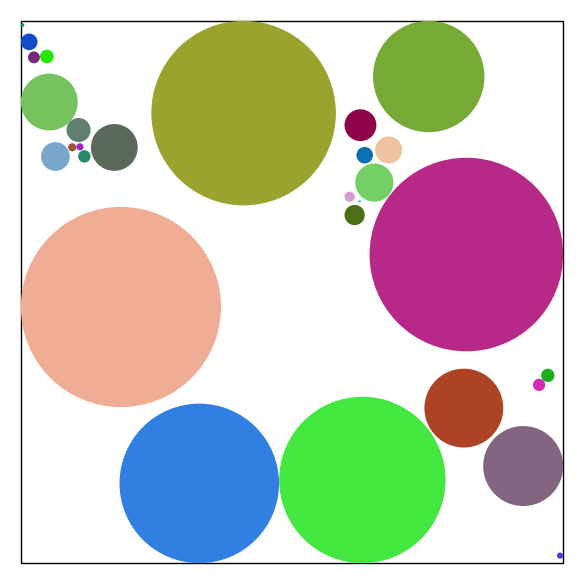
\includegraphics[width=0.5\textwidth]{square_example.png}
%    \caption{Packing of an example instance.}
%    \label{fig:example}
%\end{figure}
